\documentclass{article}

\usepackage[paperheight=10.5cm,paperwidth=10.5cm,top=0.25cm,left=0.2cm,right=0.2cm,bottom=0.25cm,
            heightrounded]{geometry}

\usepackage{xstring}
\usepackage{tikz}
\usetikzlibrary{calc}

\newcommand{\Size}{1.99cm}% Adjust size of square as desired

\def\NumOfColumns{5}%
\def\Sequence{1/A, 2/B, 3/C, 4/D, 5/E}% This needs to match \NumOfColumns 

\tikzset{Square/.style={
		inner sep=0pt,
		text width=\Size, 
		minimum size=\Size,
		draw=black,
		align=center
	}
}

% Define the contents of the cells here.
\newcommand{\NodeAA}{Pyramid}
\newcommand{\NodeAB}{Saturn}
\newcommand{\NodeAC}{Eagle}
\newcommand{\NodeAD}{Spider}
\newcommand{\NodeAE}{Soldier}

\newcommand{\NodeBA}{Time}
\newcommand{\NodeBB}{Fly}
\newcommand{\NodeBC}{Mercury}
\newcommand{\NodeBD}{Moon}
\newcommand{\NodeBE}{Model}

\newcommand{\NodeCA}{Cold}
\newcommand{\NodeCB}{Air}
\newcommand{\NodeCC}{Wake}
\newcommand{\NodeCD}{Cycle}
\newcommand{\NodeCE}{Plate}

\newcommand{\NodeDA}{Snow}
\newcommand{\NodeDB}{Angel}
\newcommand{\NodeDC}{Crane}
\newcommand{\NodeDD}{Boom}
\newcommand{\NodeDE}{Hood}

\newcommand{\NodeEA}{Torch}
\newcommand{\NodeEB}{Cat}
\newcommand{\NodeEC}{Snowman}
\newcommand{\NodeED}{Grace}
\newcommand{\NodeEE}{Spot}

\begin{document}
	\thispagestyle{empty}
	\begin{center}
	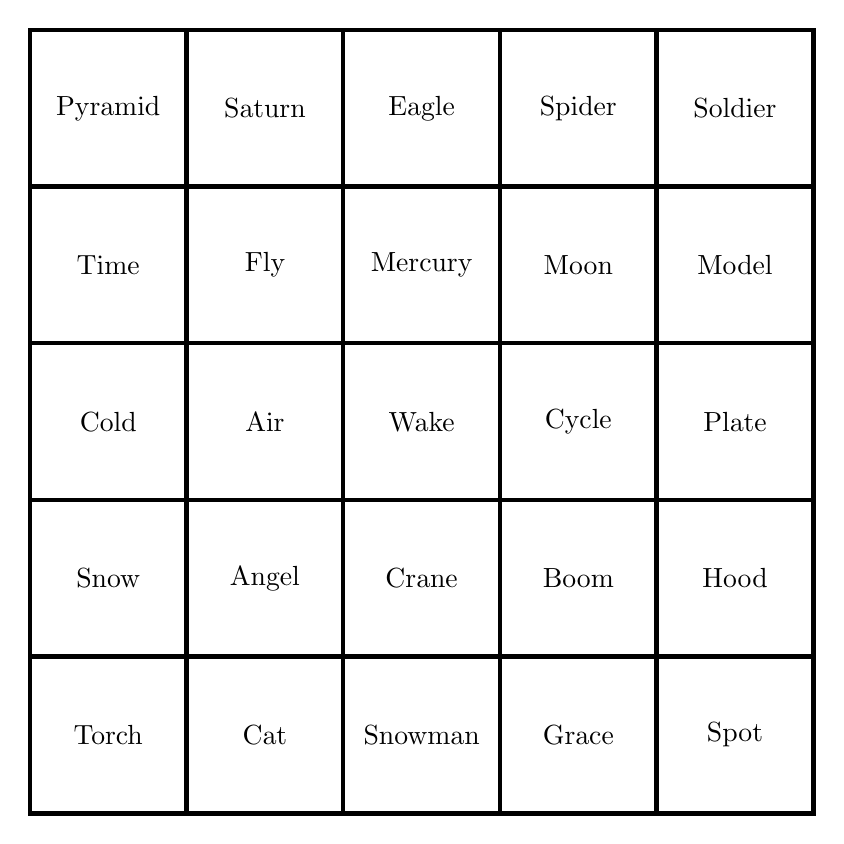
\begin{tikzpicture}[draw=black, ultra thick, x=\Size,y=\Size]
	\foreach \col/\colLetter in \Sequence {%
		\foreach \row/\rowLetter in \Sequence{%
			\pgfmathtruncatemacro{\value}{\col+\NumOfColumns*(\row-1)}
			\def\NodeText{\expandafter\csname Node\rowLetter\colLetter\endcsname}
			\node [Square] at ($(\col,-\row)-(0.5,0.5)$) {\NodeText};
		}
	}
	\end{tikzpicture}
	\end{center}
\end{document}
